\chapter{The Experimental Apparatus}
\section{The Large Hadron Collider}
The Large Hadron Collider (LHC) is a particle accelerator designed to explore the physics of particles at the energy scale of electroweak symmetry breaking. The accelerator occupies a 26.7 km tunnel beneath the Switzerland-France border near Geneva, which previously housed the Large Electron Positron Collider (LEP). Protons are accelerated in two counter-rotating beams up to a design momentum of $7~\mbox{TeV}/c$. The beams collide at four interaction points (IPs), shown in figure~\ref{fig:LHC-IPs}, where four collider detectors, ATLAS, CMS, LHCb, and ALICE, analyze the remnants of the collisions.

\begin{figure}[htbp]
	\centering
	\resizebox{0.4\textwidth}{!}{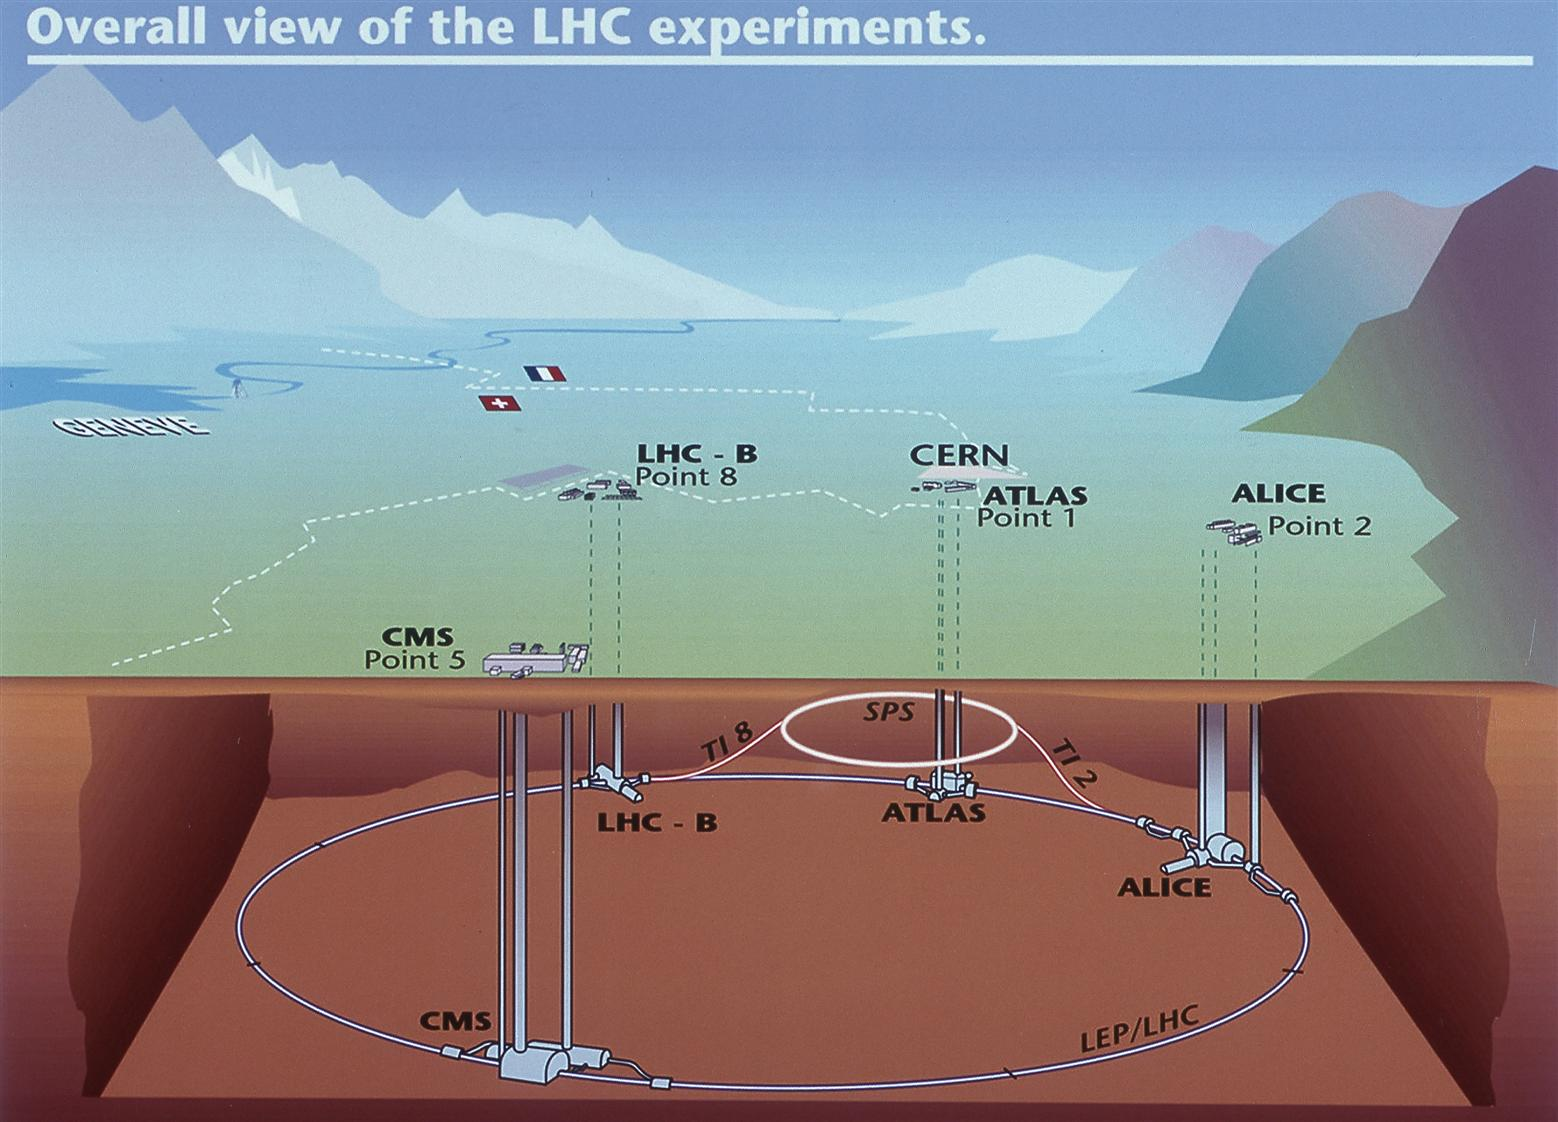
\includegraphics{figures/ch3-experiment/LHC_IPs}}
	\caption{The LHC and the four interaction points where the beams are brought into collision. The ATLAS experiment is located at interaction point 1.}
	\label{fig:LHC-IPs}
\end{figure}


The LHC project was approved in 1994 by the CERN Council, and construction proceeded over the ensuing 14 years. The collider detectors were constructed in parallel, beginning with the excavation of two additional caverns at IP1 and IP5 for the ATLAS and CMS detectors (LHCb and ALICE occupied the existing caverns at IP2 and IP8, which previously housed the DELPHI and L3 LEP experiments). The first beam was circulated on 10 September 2008; however, on 19 September, the LHC sustained severe damage due to an incident stemming from a faulty joint between magnets\footnote{A postmortem analysis implicated a bad splice between the superconducting cables of adjacent magnets as the source of the incident, with a resistance about $10^3$ times above specification. The joint melted, and 275~MJ of energy in the magnets dissipated in electric arcs, which vaporized beam pipes and breached the cryogenic vessel containing the magnets. A large amount of liquid helium entered the vacuum vessel and heated rapidly, breaking several vacuum barriers of the cryostats with a force of up to 56 tons. Ultimately, 30 dipoles and 7 quadrupoles were damaged beyond repair, and another 9 dipoles and 7 quadrupoles required repairs; 9 magnet interconnections were destroyed; 26 magnets were pushed down the tunnel; 276~MJ of energy were dissipated in electrical faults and arcs; 6 tons of helium were lost; and 2.8~km of both beam pipes were contaminated with fragments of insulation, with 1~km also contaminated with soot from molten copper and insulation.~\cite{Rossi:2010el}}. Repairs took an extra year, and the energy of the beams was reduced to $3.5-4~\mbox{TeV}$ for the first data-taking run, to mitigate the risk of another possible faulty joint. 

Proton-proton collisions at a center-of-mass energy of $\sqrt{s}=7~\mbox{TeV}$ commenced in early 2010. The LHC delivered an integrated luminosity of $\int L dt=48.1~\mbox{pb}^{-1}$ to the ATLAS detector in 2010, and $\int L dt=5.46~\mbox{fb}^{-1}$ in 2011. In 2012, the collision energy was increased to $\sqrt{s}=8~\mbox{TeV}$, and a dataset of $\int L dt=22.8~\mbox{fb}^{-1}$ was delivered. 

\subsection{The Accelerator Complex}
\begin{figure}[htbp]
	\centering
	\resizebox{3.5in}{!}{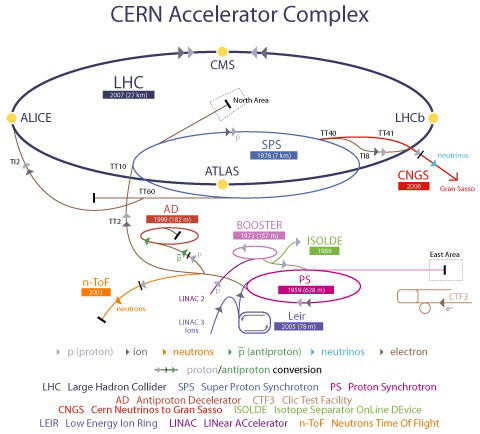
\includegraphics{figures/ch3-experiment/converted/LHC_accelerator_complex.png}}
	\caption{The LHC accelerator complex. The proton injection chain begins at LINAC2, proceeding through the booster, PS, and SPS before reaching the LHC. The facility also provides ions to the LHC, as well as a variety of particles to other experiments.}
	\label{fig:LHC-accelerator-complex}
\end{figure}


The LHC itself is the last stage of a 4-part acceleration chain, shown in figure~\ref{fig:LHC-accelerator-complex}. A full description can be found at~\cite{Benedikt:2004wm}. The staged acceleration chain meets the stringent performance requirements of the LHC, namely providing up to 2808 proton bunches with a very small transverse emittance and controllable longitudinal emittance. 

The primary devices making up the accelerators are radio frequency (RF) cavities and magnets. RF cavities are metallic structures used for particle acceleration. An example of an LHC RF cavity is shown in figure~\ref{fig:rf-cavity}. The RF cavities are driven by a power source, typically a klystron, at their resonant frequency, creating an oscillating electromagnetic field inside the structure. Proton bunches synchronized with the oscillation of the electic fields are accelerated down the cavity. 
% Talk about the bunch spacing here.

A variety of types of magnet are used to manipulate the proton beams. Dipole magnets, such as that shown in figure~\ref{fig:LHC-dipole}, provide the centripetal force that bends the beams in a circle. Quadrupole and higher order magnets focus the beams.

Protons are produced from hydrogen gas using a duoplasmatron source, which strips electrons from protons in a high electric field. After passing through a $90~\mbox{kV}$ pre-injector, a radio frequency quadrupole (RFQ) focuses and accelerates the protons to $750~\mbox{kV}$. A linear accelerator (LINAC2) then accelerates the protons to $50~\mbox{MeV}$ using RF cavities. The protons then pass through an $80~\mbox{m}$-long transfer line into the the Proton Synchrotron Booster (PSB) and Proton Synchrotron (PS). 

The PSB consists of four stacked circular synchrotrons, $157~\mbox{m}$ in circumference, and accelerates the protons to $1.4 \GeV$. The use of four separate rings mitigates the space charge effects caused by the repulsion of protons within a bunch, which scale as $N_b/(\beta\gamma^2)$, where $N_b$ is the number of protons per bunch. The protons are then injected into single-ring PS, where the higher injection energy reduces the space charge effect. The PS accelerates the beams to $25 \GeV$, and also bunches the protons in preparation for injection into the LHC. A third synchrotron in the chain, the $7~\mbox{km}$-circumference Super Proton Synchrotron (SPS), accelerates the protons to $450 \GeV$, where they are injected into the LHC. 

The protons reach a momentum of $1.4~\mbox{GeV}/c$ in the Proton Synchrotron Booster (PSB), $25~\mbox{GeV}/c$ in the Proton Synchrotron (PS), and $450~\mbox{GeV}/c$ in the Super Proton Synchrotron (SPS), before being injected into the LHC for acceleration up to the final collision energy. 


\subsection{Accelerator Parameters}
From the experiments' point of view, there are two main parameters to optimize in order to maximize sensitivity to new physics: the collision energy, $\sqrt{s}$, and the integrated luminosity, $\int L dt$. The collision energy is limited to $\sqrt{s}=14~\mbox{TeV}$ by the bending power of the dipole magnets, which have a field strength of $8.73~\mbox{T}$; however, due to the faulty splice design mentioned above, the energy was limited to $\sqrt{s}=7-8~\mbox{TeV}$ in Run I. 

The optimization of luminosity is somewhat more complicated.  The luminosity of the colliding beams is given by:
\begin{equation}\label{eqn:lumi}
	L = \frac{n_b f_r N_1 N_2 \gamma_b}{4\pi \varepsilon_n \beta_{*}},
\end{equation}
where $n_b$ is the number of colliding bunch pairs, $f_r=11245.5~\mbox{Hz}$ is the LHC revolution frequency, $N_{1,2}$ are the number of proton in the two beams, $\gamma_b$ is the relativistic gamma factor, $\varepsilon_n$ is the normalized emittance, and $\beta_{*}$ is the beta function at the collision point. TALK ABOUT THE LIMITS ON THESE NUMBERS.

In general, a higher integrated luminosity is desired; however, a high number of simultaneous collisions, $\mu=L/n_b$, can degrade the performance of the detectors. 

%\subsection{Interaction Regions}

\subsection{Run I Performance}



\section{The ATLAS Experiment}
The ATLAS detector is a large, cylindrical collider detector located at IP1 on the LHC ring (figure~\ref{fig:LHC-IPs}). The detector measures the energy and momenta of charged and colored particles produced in the collisions provided by the LHC. It consists of several subsystems occupying a cylinder , weighing (x tons). Closest to the interaction region, the inner detector performs momenta measurements of charged particles by tracking their movement through a solenoidal magnetic field (section~\ref{sec:inner-detector}). Past the inner detector solenoid magnet, electromagnetic and hadronic calorimeters measure the energy of electrons, photons, and hadrons. Finally, the muon spectrometer provides additional tracking and particle identification for muons in large toroidal magnetic field. 




\subsection{Magnets}
ATLAS relies on two powerful superconducting magnets to bend the trajectories of charged particles, allowing the tracking detectors to provide measurements of their momenta. 

% Solenoid

% Toroid


\subsection{Tracking}

\subsection{Calorimetry}

\subsection{Muon System}

\subsection{Data Acquisition}

\subsection{Data Preparation/Performance}


\printbibliography